% Queue comparison tables and replay figures before their accompanying text.
\begin{table*}[t]
    \centering
    \footnotesize
    \setlength{\tabcolsep}{5pt}
    \renewcommand{\arraystretch}{0.85}
    \caption{\textbf{Contact fidelity} on our data (video, glove, motion capture) and on GRAB. Rates in percent, pooled over anchor-frames. Millimeter columns are medians. \textbf{Bold}: best per bed and metric. \underline{Underline}: best published baseline. On GRAB we additionally compare against ReGrind ported to SHARPA Wave, which takes the GRAB mesh as input. \ours uses only the contact-reconstructed pseudo-object (\cref{fig:pseudoobject}), and the GRAB mesh only to score penetration. The glove$+$motion capture gap combines the two beds' medians weighted by anchor-frames.}
    % source: paper_metrics/out/{unified_all,grab_all}.csv; per-source breakdown in metric_results.txt
    % metrics: tart.eval.MetricAccumulator palmar_strict / region_strict / in_cone_strict / gap_med_mm / pen_med_mm
    \label{tab:contact_quality}
            \begin{tabular}{lcccccc}
        \toprule
        & \ours & DexPilot & AnyTeleop-K & AnyTeleop-P  & ReGrind & \ours \\
         & & \citep{dexpilot} & \citep{anyteleop} & \citep{anyteleop} & \citep{regrind} (w/ Object)& (init only) \\
        \midrule
        \multicolumn{7}{l}{\emph{Our data: monocular video (20 clips)}} \\
        \quad Contact rate (\%) $\uparrow$& \textbf{61.4} & \underline{9.7} & 8.3 & 7.6 & -- & 20.5 \\
        \quad Correct region (\%) $\uparrow$& \textbf{60.1} & \underline{9.5} & 8.0 & 7.5 & -- & 19.2 \\
        \quad In-cone (\%) $\uparrow$& \textbf{35.2} & 4.2 & 4.7 & \underline{5.0} & -- & -- \\
        \quad Gap (mm) $\downarrow$& \textbf{2.40} & \underline{9.99} & 10.80 & 13.19 & -- & 5.76 \\
        \midrule
        \multicolumn{7}{l}{\emph{Our data: tactile glove $+$ motion capture (66 clips)}} \\
        \quad Contact rate (\%) $\uparrow$& \textbf{77.7} & \underline{3.8} & 3.4 & 3.5 & -- & 15.9 \\
        \quad Correct region (\%) $\uparrow$& \textbf{76.9} & \underline{3.7} & 3.3 & 3.2 & -- & 15.8 \\
        \quad In-cone (\%) $\uparrow$& \textbf{46.0} & 1.1 & 1.0 & \underline{2.3} & -- & -- \\
        \quad Gap (mm) $\downarrow$& \textbf{1.38} & 17.17 & \underline{16.67} & 23.22 & -- & 9.32 \\
        \midrule
        \multicolumn{7}{l}{\emph{GRAB (100 clips)}~\citep{grab}} \\
        \quad Contact rate (\%) $\uparrow$& \textbf{43.1} & 4.9 & 4.9 &  4.6 &\underline{22.5}& 19.6 \\
        \quad Correct region (\%) $\uparrow$& \textbf{40.6} &  4.8 & 4.9 &  4.5 & \underline{20.7} & 17.8 \\
        \quad In-cone (\%) $\uparrow$& \textbf{16.2} & 1.7 & 1.7 &1.7 &\underline{5.2}&  3.8 \\
        \quad Gap (mm) $\downarrow$& \textbf{3.56} & 20.90 & 20.45 & 20.66 &  \underline{7.86}  &13.78 \\
        \quad Penetration (mm) $\downarrow$& \textbf{7.96} & 12.71 & 12.79 & 13.02 & \underline{9.80}& 11.15 \\
        \bottomrule
        \end{tabular}
\end{table*}

\begin{figure}[t]
    \centering
    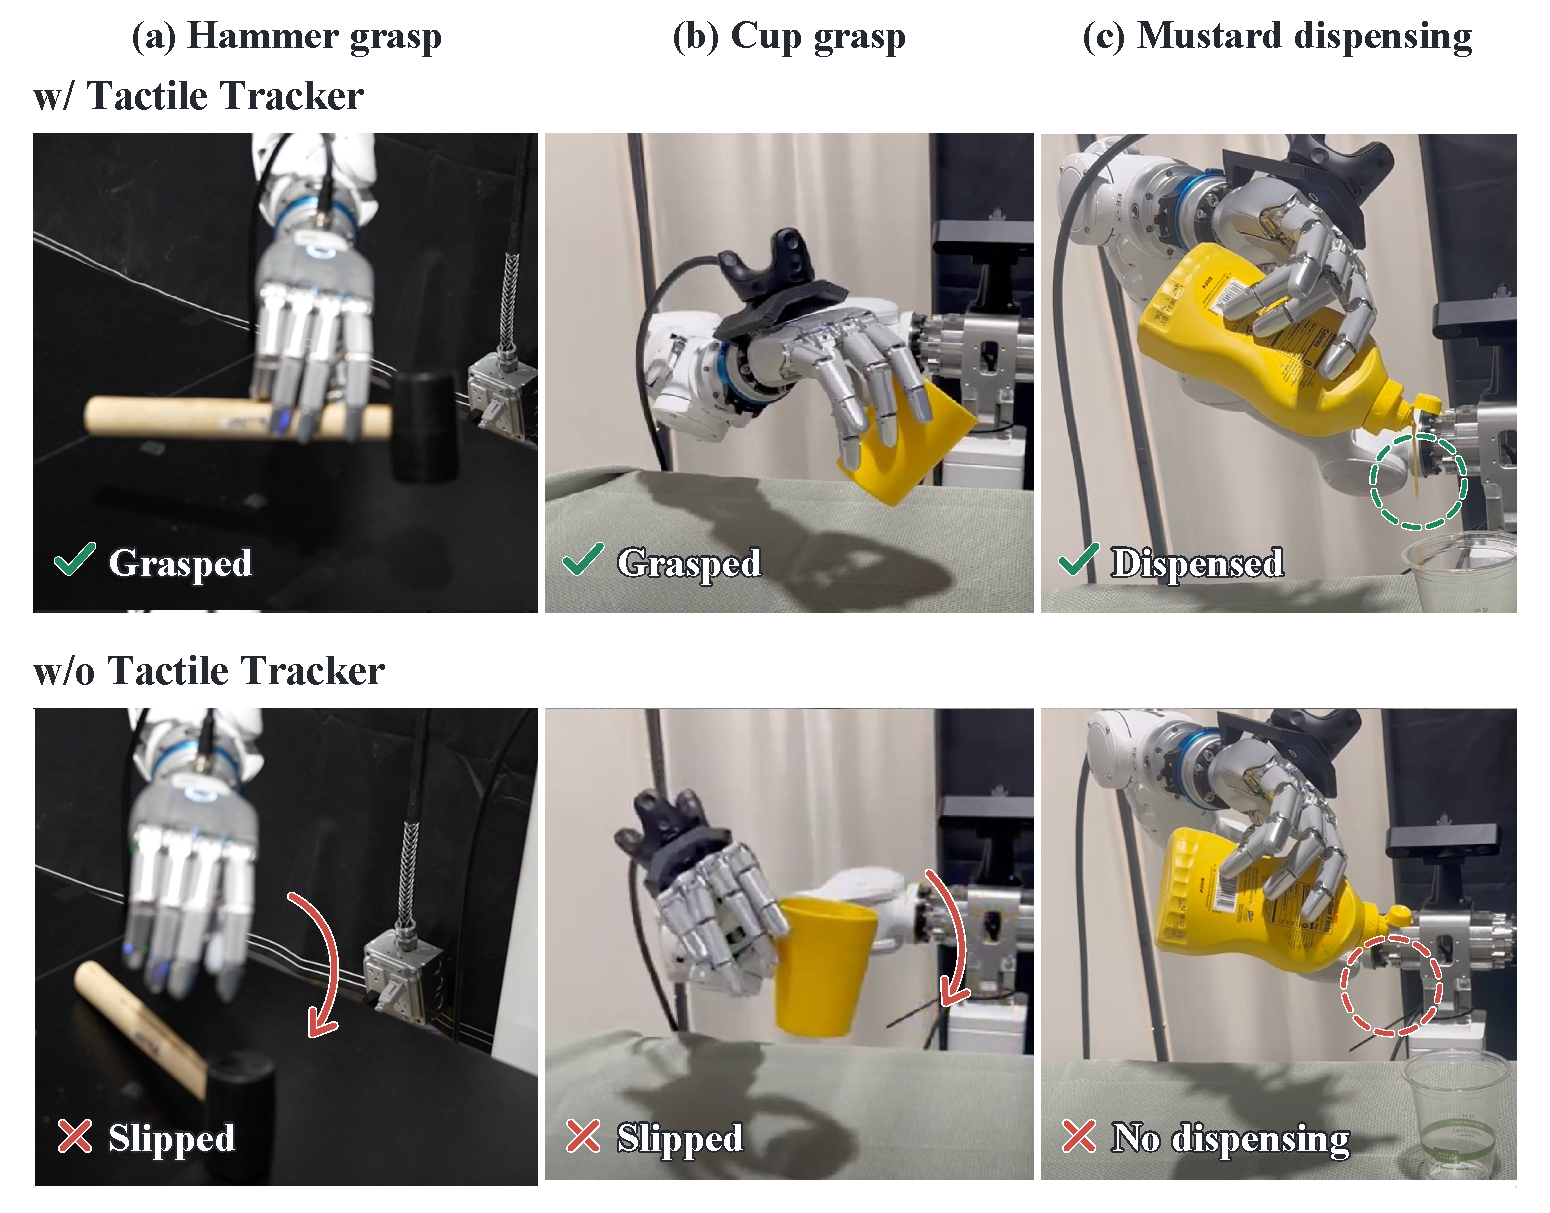
\includegraphics[width=0.8\linewidth]{figs/fig_tactile_ablation.pdf}
    \caption{\textbf{Tactile tracker ablation.} We show the same trajectories replayed with (top) and without (bottom) tactile tracking. Tactile tracking maintains the desired contact forces, enabling stable grasps and successful task execution.}

    \label{fig:tactile_ablation}
\end{figure}

\begin{figure*}[t]
    \centering
    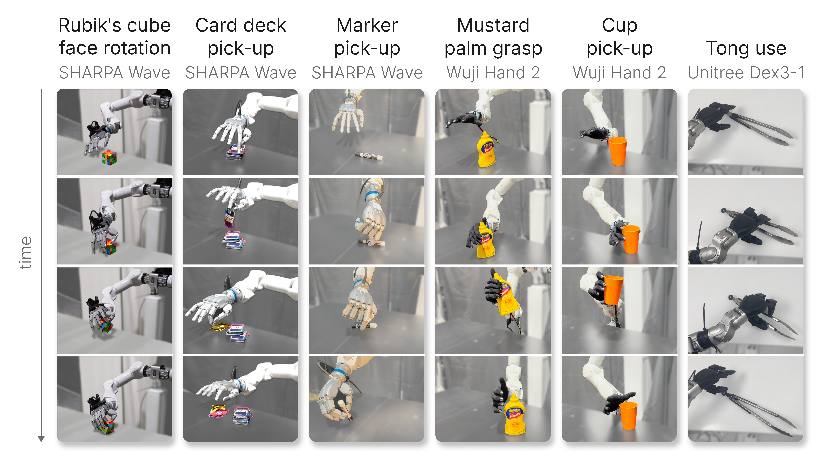
\includegraphics[width=0.9\linewidth]{figs/fig_realworld.pdf}
    \caption{\textbf{Replay on hardware.} We show a series of snapshots of \ours trajectories replayed on the SHARPA Wave hand, Wuji Hand~2, and Unitree Dex3-1.  The articulated Rubik's cube and the bending deck of cards use the same pipeline as the rigid objects.}
    \label{fig:real}
\end{figure*}

\begin{figure}[t]
    \centering
    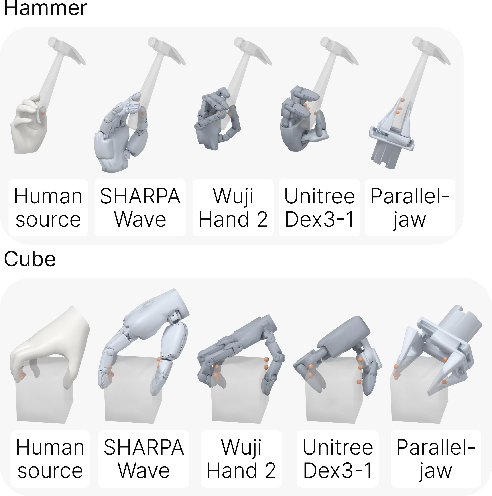
\includegraphics[width=0.8\linewidth]{figs/fig_crossemb_1col.pdf}
    \caption{\textbf{Cross-embodiment transfer.} Two GRAB demonstrations (rows) retargeted to SHARPA Wave, Wuji Hand~2, Unitree Dex3-1, and a parallel-jaw gripper (columns, after the human source). Only the semantic map changes. Orange spheres are the contact force targets.}
    \label{fig:embodiments}
\end{figure}

\begin{table}[t]
    \centering
    \caption{\textbf{Contact from monocular video.} Vid-HACO versus released HACO~\citep{haco} and HACO-R (retrained on our data), on 12-dataset validation and held-out HRDexDB~\citep{hrdexdb}. Percent, threshold 0.52 except for the threshold-free AP. Vertex metrics are pooled over all vertices and frames. Frame F1 measures whether any vertex is in contact.}
    % source: 12-dataset val -- all three models re-run 2026-10-06 on the same 172,873 hash-split samples by /data/haco12ds/code/val_ap.py; HRDexDB = /data/hrdexdb/eval/results_{vitl,haco_12ds,haco_orig}.json (eval_contact.py, thr 0.52, ego cam 25452066), summary /data/haco12ds/eval/compare_hrdexdb.md (2026-10-05).
    \label{tab:contact}
    \small
    \setlength{\tabcolsep}{4.5pt}
    \begin{tabular}{@{}lccccc@{}}
    \toprule
    & \multicolumn{4}{c}{Vertex} & Frame \\
    \cmidrule(lr){2-5}
    & F1 $\uparrow$ & Prec.\ $\uparrow$ & Rec.\ $\uparrow$ & AP $\uparrow$ & F1 $\uparrow$ \\
    \midrule
    \multicolumn{6}{@{}l}{\emph{12-dataset validation}} \\
    \quad HACO & 57.1 & 44.4 & 80.0 & 51.7 & 86.1 \\
    \quad HACO-R & 74.5 & 63.4 & \textbf{90.3} & 70.4 & 86.1 \\
    \quad Vid-HACO & \textbf{84.3} & \textbf{80.4} & 88.5 & \textbf{92.4} & \textbf{98.3} \\
    \midrule
    \multicolumn{6}{@{}l}{\emph{HRDexDB (held out)}} \\
    \quad HACO & 63.3 & 56.5 & \textbf{71.9} & 54.3 & 76.3 \\
    \quad HACO-R & 62.6 & 57.1 & 69.2 & 54.5 & 75.9 \\
    \quad Vid-HACO & \textbf{67.2} & \textbf{67.9} & 66.5 & \textbf{72.2} & \textbf{95.3} \\
    \bottomrule
    \end{tabular}\vspace{-1em}
\end{table}

\section{Experiments}
\label{sec:exp}

We evaluate \ours across five aspects: contact fidelity against kinematic baselines (\cref{sec:exp:setup}), force preservation in open-loop hardware replay (\cref{sec:exp:real}), transfer across embodiments (\cref{sec:exp:embodiment}), contact estimation from video (\cref{sec:exp:vidhaco}), and the performance of a physics-based retargeting variant, \ours--physics (\cref{sec:exp:physics}). We also provide additional ablations and contact analyses: \cref{app:ablation,app:by_source,app:contact}.

\subsection{Contact fidelity against kinematic retargeting}
\label{sec:exp:setup}

\nbf{Data} We evaluate on two datasets: clips captured in house (\cref{fig:gallery}: 20 casual phone videos, 18 tactile glove with VIVE tracker clips, and 48 motion-capture with tactile glove clips) and 100 public GRAB clips~\citep{grab} with ground-truth object meshes. Every method is retargeted to the 22-DoF SHARPA Wave.

\nbf{Metrics} A contact is considered \emph{established} when a \fcas lies within 2\,mm of the assigned link surface and the nearest pad sample is on the palmar face. \emph{Contact rate} measures the fraction of anchor-frames with established contact. \emph{Correct-region rate} further requires contact on the correct region according to the demonstration, while \emph{in-cone rate} additionally requires the pad normal to align within $45^\circ$ of the demonstrated push direction. \emph{Gap} is the median distance from the contact force target to the pad and \emph{penetration} the median deepest incursion into the object (\cref{app:metrics}).

\nbf{Baselines} We compare against the kinematic retargeting baselines: DexPilot~\citep{dexpilot} and the two objectives of AnyTeleop~\citep{anyteleop}, key-vector (AnyTeleop-K) and fingertip-position (AnyTeleop-P). We also report ReGrind~\citep{regrind} (w/ Object), a contact-preserving retargeting method that requires the object mesh, and \ours's geometric initialization (init only). TopoRetarget~\citep{toporetarget} and Morphometric Imitation~\citep{morphometric} have not released code at submission time and are therefore not compared.

\nbf{Results} \Cref{tab:contact_quality} compares contact fidelity across both datasets. Kinematic baselines establish the demonstrated contact on only 3--10\% of anchor-frames, with a median gap of 10--23\,mm. In contrast, \ours establishes contact on 61\% of anchor-frames on video, 78\% on the glove and motion-capture clips, and 43\% on GRAB, while reducing the gap to 1.4--3.6\,mm. Importantly, nearly all established contacts occur on the correct finger, and over half of anchor-frames also satisfy the in-cone constraint. On GRAB, where ground-truth object meshes allow us to measure penetration, \ours reaches 43\% contact against 22.5\% for ReGrind, which takes the object mesh as input, and also produces the least object penetration (7.96\,mm) (\cref{fig:baselines}). We also find that contact fidelity correlates with contact signal quality: \ours can achieve 89\% contact on the tactile glove clips, where contact is measured, 76\% on motion capture, 61\% on video, where it is inferred, and 43\% on GRAB, where contact is calculated from geometric proximity (\cref{app:by_source}).

\subsection{Open-loop replay on hardware}
\label{sec:exp:real}

To directly evaluate the fidelity of \ours's retargeted actions, we replay the trajectories open-loop on real hardware, eliminating confounding factors such as policy learning. Under this setting, task success depends directly on the faithful reproduction of task-critical contacts and forces. \cref{fig:real} shows sequential snapshots of our hardware replays, including picking up a deformable card from a deck and rotating an articulated Rubik’s Cube with a single finger. All tasks use our tactile tracking controller to preserve contact forces. Full videos are available on our project website.

\nbf{Tactile tracker ablation} We replay identical \ours trajectories on the SHARPA Wave with and without the tactile tracker on three real-world tasks, 10 trials each (\cref{fig:tactile_ablation}). Position-only replay succeeds on 1/10 hammer lifts, 3/10 cup lifts, and 0/10 mustard dispenses: the hammer and cup slip out during the lift while the bottle is lifted but not squeezed. With the tactile tracker the same trajectories succeed on 8/10, 10/10, and 7/10 respectively. Reproducing the joint motion alone does not reproduce the intended contact forces.


\subsection{Cross-embodiment transfer}
\label{sec:exp:embodiment}

Here we demonstrate that the same \fca formulation can retarget to new embodiments such as the Wuji Hand~2, the Unitree Dex3-1 and a parallel-jaw gripper (\cref{fig:embodiments}) by only changing the semantic mapping. Specifically, we show hardware rollouts with the first two embodiments in \cref{fig:real}. Unitree Dex3-1 has no tactile sensing, so we scale its grasp actions 1.2$\times$. Although the Wuji Hand~2 also has no tactile sensing, we found that it needs no scaling, since its compliant inner surfaces conform to the object.



\subsection{Contact estimation from video}
\label{sec:exp:vidhaco}

\nbf{Setup} We compare our video contact model Vid-HACO with HACO~\citep{haco} and HACO-R, HACO retrained on the same 12-dataset training set as ours. We evaluate on the $\sim$173k-frame validation split and held-out HRDexDB~\citep{hrdexdb}: 434 egocentric videos of 94 objects (111.9k frames). All models use identical hand crops, the 10\,mm contact rule, and threshold 0.52.

\nbf{Results} \Cref{tab:contact} shows that Vid-HACO achieves 84.3 vertex F1 on validation and 67.2 on HRDexDB, improving held-out F1 by 3.9 points over released HACO. Retraining HACO improves validation F1 to 74.5 but leaves held-out F1 at 62.6. Vid-HACO exceeds this matched-data baseline by 4.6 F1 and 17.7 AP. Frame F1 reaches 95.3 versus 75.9 for both baselines, which predict contact on every frame. This is important for retargeting since hallucinated contacts during a reach can pull robot fingers toward empty space. Further analysis is provided in \cref{app:contact}.

\subsection{\ours with physically plausible retargeting}
\label{sec:exp:physics}

\begin{table}[t]
    \centering
    \small
    \setlength{\tabcolsep}{8pt}
    \caption{\textbf{\ours-physics.} We compare \ours-physics, our physics retargeting variant, against SPIDER's physics stage~\citep{spider}. Strict task success in percent on 48 motion-capture demonstrations (2 seeds) and 50 GRAB clips (1 seed). A task counts as solved when at least one seed succeeds (\cref{app:physics}).}
    % source (fhshare worktree): docs/results_spider_vs_card.md "Main comparison" (2026-10-22, MAX_ERR 0.15 m): Mocap-50 A 20/50 F 26/50; GRAB-50 A 6/50 F 16/50
    \label{tab:physics}
    \begin{tabular}{lcc}
        \toprule
        & Motion capture (48) & GRAB (50) \\
        \midrule
        SPIDER~\citep{spider} & 40\% & 12\% \\
        \ours-physics & \textbf{52\%} & \textbf{32\%} \\
        \bottomrule
    \end{tabular}\vspace{-1em}
\end{table}


We further test whether \fca and the contact objective improve physics-based retargeting. We build \ours-physics on SPIDER~\citep{spider}, a simulation-based retargeting framework that tracks kinematic references using a sampling-based optimization solver. \ours-physics modifies SPIDER in three ways: (1) initialize from \ours's retargeted trajectories, (2) replace SPIDER's contact-guidance term with our contact objective $E_{\mathrm{contact}}(q)$, and (3) extract \fca using our pipeline (details and weights in \cref{app:physics}).

We evaluate on 50 GRAB and 48 motion-capture trajectories with ground-truth contact, object meshes, and object trajectories. \ours-physics raises strict task success from 12\% to 32\% on GRAB and from 40\% to 52\% on motion capture (\cref{tab:physics}), showing evidence that our contact representation also benefits physics-based retargeting.
%===============================================================================
